%%%%%%%%%%%%%%%%%%%%%%%%%%%%%%%%%%%%%%%%
% Structured General Purpose Assignment
% LaTeX Template
%
% This template has been downloaded from:
% http://www.latextemplates.com
%
% Original author:
% Ted Pavlic (http://www.tedpavlic.com)
%
% Note:
% The \lipsum[#] commands throughout this template generate dummy text
% to fill the template out. These commands should all be removed when 
% writing assignment content.
%
%%%%%%%%%%%%%%%%%%%%%%%%%%%%%%%%%%%%%%%%%

%----------------------------------------------------------------------------------------
%       PACKAGES AND OTHER DOCUMENT CONFIGURATIONS
%----------------------------------------------------------------------------------------

\documentclass{article}

\usepackage{fancyhdr} % Required for custom headers
\usepackage{lastpage} % Required to determine the last page for the footer
\usepackage{extramarks} % Required for headers and footers
\usepackage{graphicx} % Required to insert images
\usepackage{lipsum} % Used for inserting dummy 'Lorem ipsum' text into the template

\usepackage{amsmath}
    \usepackage{todonotes}

% Margins
\topmargin=-0.45in
\evensidemargin=0in
\oddsidemargin=0in
\textwidth=6.5in
\textheight=9.0in
\headsep=0.25in 

\linespread{1.1} % Line spacing

% Set up the header and footer
\pagestyle{fancy}
\lhead{\hmwkAuthorName} % Top left header
\chead{\hmwkClass\ : \hmwkTitle} % Top center header
\rhead{\firstxmark} % Top right header
\lfoot{\lastxmark} % Bottom left footer
\cfoot{} % Bottom center footer
\rfoot{Page\ \thepage\ of\ \pageref{LastPage}} % Bottom right footer
\renewcommand\headrulewidth{0.4pt} % Size of the header rule
\renewcommand\footrulewidth{0.4pt} % Size of the footer rule

\setlength\parindent{0pt} % Removes all indentation from paragraphs

%----------------------------------------------------------------------------------------
%       DOCUMENT STRUCTURE COMMANDS
%       Skip this unless you know what you're doing
%----------------------------------------------------------------------------------------

% Header and footer for when a page split occurs within a problem environment
\newcommand{\enterProblemHeader}[1]{
\nobreak\extramarks{#1}{#1 continued on next page\ldots}\nobreak
\nobreak\extramarks{#1 (continued)}{#1 continued on next page\ldots}\nobreak
}

% Header and footer for when a page split occurs between problem environments
\newcommand{\exitProblemHeader}[1]{
\nobreak\extramarks{#1 (continued)}{#1 continued on next page\ldots}\nobreak
\nobreak\extramarks{#1}{}\nobreak
}

\setcounter{secnumdepth}{0} % Removes default section numbers
\newcounter{homeworkProblemCounter} % Creates a counter to keep track of the number of problems

\newcommand{\homeworkProblemName}{}
\newenvironment{homeworkProblem}[1][Problem \arabic{homeworkProblemCounter}]{ % Makes a new environment called homeworkProblem which takes 1 argument (custom name) but the default is "Problem #"
\stepcounter{homeworkProblemCounter} % Increase counter for number of problems
\renewcommand{\homeworkProblemName}{#1} % Assign \homeworkProblemName the name of the problem
\section{\homeworkProblemName} % Make a section in the document with the custom problem count
\enterProblemHeader{\homeworkProblemName} % Header and footer within the environment
}{
\exitProblemHeader{\homeworkProblemName} % Header and footer after the environment
}

\newcommand{\problemAnswer}[1]{ % Defines the problem answer command with the content as the only argument
\noindent\framebox[\columnwidth][c]{\begin{minipage}{0.98\columnwidth}#1\end{minipage}} % Makes the box around the problem answer and puts the content inside
}

\newcommand{\homeworkSectionName}{}
\newenvironment{homeworkSection}[1]{ % New environment for sections within homework problems, takes 1 argument - the name of the section
\renewcommand{\homeworkSectionName}{#1} % Assign \homeworkSectionName to the name of the section from the environment argument
\subsection{\homeworkSectionName} % Make a subsection with the custom name of the subsection
\enterProblemHeader{\homeworkProblemName\ [\homeworkSectionName]} % Header and footer within the environment
}{
\enterProblemHeader{\homeworkProblemName} % Header and footer after the environment
}
   
%----------------------------------------------------------------------------------------
%       NAME AND CLASS SECTION
%----------------------------------------------------------------------------------------

\newcommand{\hmwkTitle}{Assignment\ \# 2} % Assignment title
\newcommand{\hmwkDueDate}{Friday,\ October\ 2,\ 2015} % Due date
\newcommand{\hmwkClass}{CSCI-567} % Course/class
\newcommand{\hmwkClassTime}{} % Class/lecture time
\newcommand{\hmwkAuthorName}{Saket Choudhary} % Your name
\newcommand{\hmwkAuthorID}{2170058637} % Teacher/lecturer
%----------------------------------------------------------------------------------------
%       TITLE PAGE
%----------------------------------------------------------------------------------------

\title{
\vspace{2in}
\textmd{\textbf{\hmwkClass:\ \hmwkTitle}}\\
\normalsize\vspace{0.1in}\small{Due\ on\ \hmwkDueDate}\\
\vspace{0.1in}\large{\textit{\hmwkClassTime}}
\vspace{3in}
}

\author{\textbf{\hmwkAuthorName} \\
        \textbf{\hmwkAuthorID}
        }
\date{} % Insert date here if you want it to appear below your name

%----------------------------------------------------------------------------------------

\begin{document}

\maketitle

%----------------------------------------------------------------------------------------
%       TABLE OF CONTENTS
%----------------------------------------------------------------------------------------

%\setcounter{tocdepth}{1} % Uncomment this line if you don't want subsections listed in the ToC

\newpage
\tableofcontents
\newpage
 \listoftodos

%----------------------------------------------------------------------------------------
%       PROBLEM 2
%----------------------------------------------------------------------------------------

\begin{homeworkProblem}[Problem 1] % Custom section title


\begin{homeworkSection}{\homeworkProblemName: ~(a)}
\problemAnswer{ % Answer
Linear regression assumes uncertainty in th measurement of dependent variables($Y$). $X$ being an independent variable is assumed to be the 'true' value that can be measured with ultimate precision. Any model that relates the independent variable to dependent will assume some kind of modeling error which in case of linear regression is often taken as Gaussian random variable . Additively the 'noise' and the independent variable predict the dependent. 

%\todo{Fix this answeer. it is verbose}

}
\end{homeworkSection}


\begin{homeworkSection}{\homeworkProblemName: ~(b)}
	\problemAnswer{ % Answer
		In order to make linear regression robust to outliers, a n\"{a}ive solution will choose "absolute deviation"($L1$ norm) over "squared error"($L2$ norm) as the criterion for loss function. The reason this might work out in most cases(especially when the outliers belong to a non normal distribution) is that "squared error" will blow up errors when they are large. Thus $L2$ norm will give more weight to large residuals($|y-w^Tx|^2>>|y-w^Tx|$ and we are trying to minimise this error), while the $L1$ norm gives equal weights to all  residuals.
	}
\end{homeworkSection}


\begin{homeworkSection}{\homeworkProblemName: ~(c)}
	\problemAnswer{ % Answer
		A quick way to realise this is to consider the scale. Say one of the dependent variables is 'time'. Rescaling time from hours to seconds will also rescale its coefficient, but the importance remains the same!
		
		Another example is to consider a model with two dependent variables that affect the dependent variable in a similar manner. However 
		they are on different scales say $X1$ on [1-100] and $X2$ on [0-1], resulting in the coefficient of $X1$ being too smaller than that of $X2$
		in a linear regression setting.
	}
\end{homeworkSection}

\begin{homeworkSection}{\homeworkProblemName: ~(d)}
	\problemAnswer{ % Answer
		If the dependent variables are perfect linear combination, the matrix $XX^T$ will be non invertible.
	}
\end{homeworkSection}

\begin{homeworkSection}{\homeworkProblemName: ~(e)}
	\problemAnswer{ % Answer
		A simple solution would be to use $k-1$ bits instead of $k$ bits for k categories. For example, using the following setup for a 3 category setup:
		\begin{align*}
			Red &= 0 0\\
			Green &= 1 0\\
			Blue &= 0 1
		\end{align*}
	}
\end{homeworkSection}

\begin{homeworkSection}{\homeworkProblemName: ~(f)}
	\problemAnswer{ % Answer
		If the independent variables are highly correlated, the coefficients might still be entirely different. From the example in Part (c) abov
	}
\end{homeworkSection}

\begin{homeworkSection}{\homeworkProblemName: ~(g)}
	\problemAnswer{ % Answer
		Using a posterior probability cutoff of 0.5 in linear regression is not same as 0.5 for logistic. A 0.5 rehsold on logistic guarantees that the point all points lying to the right belong to one class. However for a regression problem, this is not true, because the predicted value of $y$ is an 'intepolated or extraplolated' 
		In any case, logistic regression is a better choice, since the output is constrained in the range of $0-1$, which can be treated directly as a probability values as compared to the less intuitive relation with the output of the linear regression. 

	}
\end{homeworkSection}

\begin{homeworkSection}{\homeworkProblemName: ~(h)}
	\problemAnswer{ % Answer
		When the number of variables exceed the number of samples, the system is undetermined. And yes, it can be solved by simply obtaining psuedo-inverse of $X$ which is always defined.
	}
\end{homeworkSection}

\end{homeworkProblem}

\begin{homeworkProblem}[Problem 2]
\begin{homeworkSection}{\homeworkProblemName: ~(a)}
	\problemAnswer{
		Class 1: $\vec{x} = (x_1, x_2, \cdots x_{2D})$ where each $x_i \sim N(0, \sigma^2)$
		
		Class 2: $\vec{x} = (x_1, x_2, \cdots x_D, x_{D+1}+\delta, \cdots x_{2D})$
		
		From first principles, the discriminant curve is given by:
		$$
		P(y=1|x) \geq P(y=0|x)
		$$
		
		And hence we have:
		
		\begin{align*}
		\log(P(y=1|x)) &\geq \log(P(y=0|x))\\
		\log(P(x|y=1)p(y=1) &\geq \log(P(x|y=0)p(y=0)\\
		\tag{1}\log(P(x|y=1))+\log(P(y=1)) &\geq \log(P(x|y=0)) + \log(p(y=0))\\
		\end{align*}
		
		Now, since $x$ is 2D dimensional and assuming independece of all attributes:
		\begin{align*}
		P(x|y=1) &= \prod_{i=1}^{2D} p(x_i|y=1) \\
		\log(P(x|y=1) &= \sum_{i=1}^{2D} \log(p(x_i|y=1))\\
		\log(P(x|y=1)) &= -{D}\log(2\pi \sigma^2) -\sum_{i=1}^{2D}\frac{x_i^2}{2\sigma^2}\tag{2}
		\end{align*}
		
		Similarly for class $0$: $x_i \sim N(0, \sigma^2) \forall x \in \{1..D\}$ and 
		 $x_i \sim N(\delta, \sigma^2) \forall x \in \{D+1..2D\}$
			\begin{align*}
			P(x|y=0) &= \prod_{i=1}^{2D} p(x_i|y=0) \\
			\log(P(x|y=0) &= \sum_{i=1}^{D} \log(p(x_i|y=1)) +\sum_{i=1}^{D} \log(p(x_i|y=1) \\
			\log(P(x|y=0)) &= -{D}\log(2\pi \sigma^2) -\sum_{i=1}^{D}\frac{x_i^2}{2\sigma^2} - \sum_{i=D+1}^{2D}\frac{(x_i-\delta)^2}{2\sigma^2}\tag{3}
			\end{align*}

		
}
\clearpage
\problemAnswer{
 		
 		Plugging $(2),(3)$ in $(1)$ we get:
 		\begin{align*}
	 	-D\log(2\pi \sigma^2) -\sum_{i=1}^{2D}\frac{x_i^2}{2\sigma^2} + \log(p(y=1)) &\geq -D\log(2\pi \sigma^2) -\sum_{i=1}^{D}\frac{x_i^2}{2\sigma^2} - \sum_{i=D+1}^{2D}\frac{(x_i-\delta)^2}{2\sigma^2} + \log(p(y=0))\\
	 	 \log(p(y=1)) +  -\sum_{i=D+1}^{2D}\frac{x_i^2}{2\sigma^2} &\geq - \sum_{i=D+1}^{2D}\frac{x_i^2-2\delta x_i + \delta^2}{2\sigma^2} + \log(p(y=0))\\
	 	 \log(p(y=1))-\log(p(y=0)) &\geq \frac{D\delta}{\sigma^2} \sum_{i=D+1}^{2D}x_i - D\frac{\delta^2}{2\sigma^2}\\
	 	 \log(p(y=1))-\log(p(y=0)) &\geq \frac{D\delta}{\sigma^2} \sum_{i=1}^{D}x_i - D\frac{\delta^2}{2\sigma^2}\\
	 	 -\frac{D\delta}{\sigma^2} \sum_{i=1}^{D}x_i + D\frac{\delta^2}{2\sigma^2} &+ \log(p(y=1))-\log(p(y=0)) \geq 0
 		\end{align*} 
 		Where the change of indices in the penultimate step is permitted since $x_i$ are i.i.d(after taking care of the shifted mean)
 		
 		Now consider the general form solution of LDA and GDA:
 		
 		\begin{align*}
 		\sum_i b_i x_i + c &\geq 0\tag{LDA}\\
 		\sum_i a_ix_i^2 + \sum b_i x_i + c &\geq 0\tag{GDA}
 		\end{align*}
		
		Where $x_i$ represents the $i^{th}$ dimension indepdent variable, where each $x_i$ is a feature/attribute and hence is not limited to 2 dimensional special case.
		
		In this case, owing to the homoscedasticity assumption(the variance of the two class conditions being equal to $\sigma^2$) LDA and GDA return the same solution.
		
		\underline{Solution form for $LDA$:}
		
		\begin{align*}
			-\frac{D\delta}{\sigma^2} \sum_{i=1}^{D}x_i + D\frac{\delta^2}{2\sigma^2} &+ \log(p(y=1))-\log(p(y=0)) \geq 0
		\end{align*}
		
		Assuming equal priors, $p(y=1) = p(y=0)$,
		
		\begin{align*}
		-\frac{D\delta}{\sigma^2} \sum_{i=1}^{D}x_i + D\frac{\delta^2}{2\sigma^2} \geq 0 \\
		 -\sum_{i=1}^{D}x_i + \frac{\delta}{2} \geq 0
		\end{align*}
		
		and hence for LDA $b_i = 0 \forall i \in \{1..D\}$ and  $b_i = -\frac{D\delta}{\sigma^2} \forall i \in \{D+1..2D\}$(simpliifies to $-1$ for the case with equal priors). and $c = \frac{D\delta^2}{2\sigma^2}$ (simplifies to $\frac{\delta}{2}$ for the case with equal priors )
		
		\textbf{In either case it does depend on $\delta$}
		
		\underline{Solution for $GDA$}:
			\begin{align*}
			-\frac{D\delta}{\sigma^2} \sum_{i=1}^{D}x_i + D\frac{\delta^2}{2\sigma^2} &+ \log(p(y=1))-\log(p(y=0)) \geq 0
			\end{align*}
			
			and hence $a_i = 0 \forall i$ and $b_i = 0 \forall i \in \{1..D\}$ and  $b_i = -\frac{D\delta}{\sigma^2} \forall i \in \{D+1..2D\}$(simplifies to $-1$ for the case with equal priors).
			
		\textbf{In either case it does depend on $\delta$}
}
\end{homeworkSection}
\begin{homeworkSection}{\homeworkProblemName: ~(b1)}
	\problemAnswer{
		$P(X|Y=c_1) \sim N(\mu_1, \Sigma)$ and $p(X|Y=c_2) \sim N(\mu_2, \Sigma)$
		
		where $\mu_1, \mu_2 \in R^D, \Sigma \in R^{D\times D}$
		
		\begin{align*}
		P(Y=1|X) &= \frac{P(X|Y=1)P(Y=1)}{P(X)}\\
		&= \frac{P(X|Y=1)P(Y=1)}{P(X|Y=1)P(Y=1)+P(X|Y=2)P(Y=2)}\\
		&= \frac{1}{1+\frac{P(X|Y=2)P(Y=2)}{P(X|Y=1)P(Y=1)}}\\
		&= \frac{1}{1+\exp(\log(\frac{P(X|Y=2)P(Y=2)}{P(X|Y=1)P(Y=1)}))}\\
		&= \frac{1}{1+\exp(\log({P(X|Y=2)P(Y=2)})-\log({P(X|Y=1)P(Y=1)}))}\\
		&= \frac{1}{1+\exp(-(\log(\frac{P(Y=1)}{P(Y=2)}))+\log(P(X|Y=2))-\log(P(X|Y=1)))}\tag{4}\\
		\end{align*}
		
		\begin{align*}
		\log(P(X|Y=1)) &= -\frac{1}{2} \ln(|\Sigma|) - \frac{D}{2}\ln(\pi) -\frac{1}{2}(x-\mu_1)^T\Sigma^{-1}(x-\mu_1)\\ 
		\log(P(X|Y=2)) &= -\frac{1}{2} \ln(|\Sigma|) - \frac{D}{2}\ln(\pi) -\frac{1}{2}(x-\mu_2)^T\Sigma^{-1}(x-\mu_2)\\
		\log(P(X|Y=2))-\log(P(X|Y=1)) &= \frac{1}{2}(x-\mu_1)^T\Sigma^{-1}(x-\mu_1) - \frac{1}{2}(x-\mu_2)^T\Sigma^{-1}(x-\mu_2)\\
		\log(P(X|Y=2))-\log(P(X|Y=1)) &= (\mu_1^T-\mu_2^T)\Sigma^{-1}x + x^T\Sigma^{-1}(\mu_1-\mu_2)\\
		\log(P(X|Y=2))-\log(P(X|Y=1)) &= 2(\mu_1^T-\mu_2^T)\Sigma^{-1}x
		\end{align*}
		
		Plugging $(5)$ in $4$:
		\begin{align*}
		P(Y=1|X) &= \frac{1}{1+\exp(-(\log(\frac{P(Y=1)}{P(Y=2)})+2(\mu_1^T-\mu_2^T)\Sigma^{-1}x  ))}\\
		P(Y=1|X) &= \frac{1}{1+\exp(-(C+\theta^T x  ))}
		\end{align*}
		
		Where $C = \frac{P(Y=1)}{P(Y=2)}$
		
		$\theta = 2(\mu_1-\mu_2)\Sigma^{-1}$ (since $(\Sigma^{-1})^T = \Sigma^{-1}$)
	
	
		 
	}
\end{homeworkSection}

\begin{homeworkSection}{\homeworkProblemName: ~(b2)}
	\problemAnswer{
		
		Given $p(y|x)$ is logistic
		$P(Y=1|X) = \frac{1}{1+\exp(-(C+\theta^T x  ))}$
		
		Consider the simplification using first principles as in part(b1):
		
		\begin{align*} 
		P(Y=1|X)&= \frac{1}{1+\exp(-(\log(\frac{P(Y=1)}{P(Y=2)}))+\log(P(X|Y=2))-\log(P(X|Y=1)))}
		\end{align*}
		
		Now, consider the distribution $P(X=x|Y=1) = e^{-\lambda_1} \frac{\lambda_1^x}{x!}$ and
		$P(X=x|Y=2) = e^{-\lambda_2} \frac{\lambda_2^x}{x!}$ 
		
		$\log(P(X|Y=2))-\log(P(X|Y=1) = \lambda_1-\lambda_2 +x(log\frac{\lambda_1}{\lambda_2})$
		
		and hence,
		
		\begin{align*} 
		P(Y=1|X) &= \frac{1}{1+\exp(-(\log(\frac{P(Y=1)}{P(Y=2)}))+\lambda_1-\lambda_2 +x(log\frac{\lambda_1}{\lambda_2}) ))}
		\end{align*}
		implying it is possible to arrive at a logistic regression expression even from a poisson distribution and hence the $p(x|y)$ need not be gaussian.
	
		}
\end{homeworkSection}

\end{homeworkProblem}

\begin{homeworkProblem}{3}
\problemAnswer{
	\begin{align*}
		L(w_{i+1}, \lambda) &=  ||w_{i+1}-w_i||_2^2+ \lambda(w_{i+1}^Tx_i)y_i\\
		&= (w_{i+1}-w_i)^T(w_{i+1}-w_i) + \lambda(w_{i+1})\\
		\Delta_{w_{i+1}} L &= 2w_{i+1}-2w_i + \lambda x_iy_i = 0 \tag{3.1} \\
		\Delta_{\lambda} L &=  w_{i+1}^Tx_iy_i = 0 \tag{3.2} \\
	\end{align*}
	
	Thus, from $3.1$ and $3.2$,
	\begin{align*}
		w_{i+1} &= w_i - \frac{1}{2}\lambda x_i\\
		&\text {where} \\
		w_{i+1}^Tx_iy_i = 0
	\end{align*}
	}
\end{homeworkProblem}



\begin{homeworkProblem}{4}
	\begin{homeworkSection}{\homeworkProblemName: ~(a)}
			\begin{tabular}{|c|c|}
				\hline Variable  & $\# Missing$ \\ 
				\hline pclass & 0  \\ 
				\hline survival & 0 \\ 
				\hline name & 0 \\ 
				\hline sex & 0 \\ 
				\hline age & 263  \\ 
				\hline sibsp  & 0 \\ 
				\hline parch & 0 \\ 
				\hline ticket & 0  \\ 
				\hline fare & 1  \\ 
				\hline cabin & 1014  \\ 
				\hline embarked & 2 \\ 
				\hline boat & 823 \\ 
				\hline body & 1188 \\ 
				\hline home & 564 \\ 
				\hline 
			\end{tabular} 

	\end{homeworkSection}
	
\begin{homeworkSection}{\homeworkProblemName: ~(b)}
	\begin{figure}
	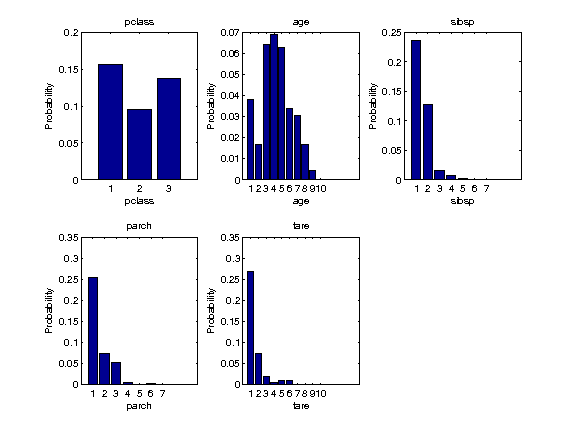
\includegraphics{data/problem4b}
	\caption{4a. Montonic relationship}
	\end{figure}
	
	From the graph above we see that  $pclass$ might not be a really informative.

\end{homeworkSection}
\begin{homeworkSection}{\homeworkProblemName: ~(c)}
	\problemAnswer{
\begin{tabular}{|c|c|}
	\hline Variable  & Information \\ 
	\hline home & 0.999467 \\ 
	\hline name & 0.963746 \\ 
	\hline sex & 0.963746 \\ 
	\hline ticket & 0.963746  \\ 
	\hline embarked & 0.963129 \\ 
	\hline cabin & 0.940286  \\
	\hline fare & 0.493161  \\  
	\hline boat & 0.095333 \\ 
	\hline pclass & 0.066290  \\ 
	\hline parch & 0.034475 \\ 
	\hline age & 0.026518  \\ 
	\hline sibsp  & 0.012308 \\ 
	\hline body & 0.00 \\ 
	\hline 
\end{tabular} 
}
\end{homeworkSection}	

\begin{homeworkSection}{\homeworkProblemName: ~(d)}
\problemAnswer{
		MM: Multiple Models\\
		SM: Substituted Models
	
	
		\begin{tabular}{|c|c|c|c|}
			\hline & With age column(MM) & Without Age column(MM) & With NaN substituted(SM) \\
			\hline Testing Accuracy & 0.776758 & 0.801223 & 0.776758 \\
			\hline Training Accuracy & 0.769466 & 0.781679 &  0.775573\\ 
			\hline 
		\end{tabular} 
		
		Thus, the multiple models with the age column completely removed seems to have worked better. This is an indicative that the 'age' factor is not really informative as is also evident from part (c) above where 'age' features low in the information table.
	}
\end{homeworkSection}

\begin{homeworkSection}{\homeworkProblemName: ~(e)}
\problemAnswer{
	Total number of columns: $602$.
	}
\end{homeworkSection}

\begin{homeworkSection}{\homeworkProblemName: ~(f)}
	\begin{figure}
		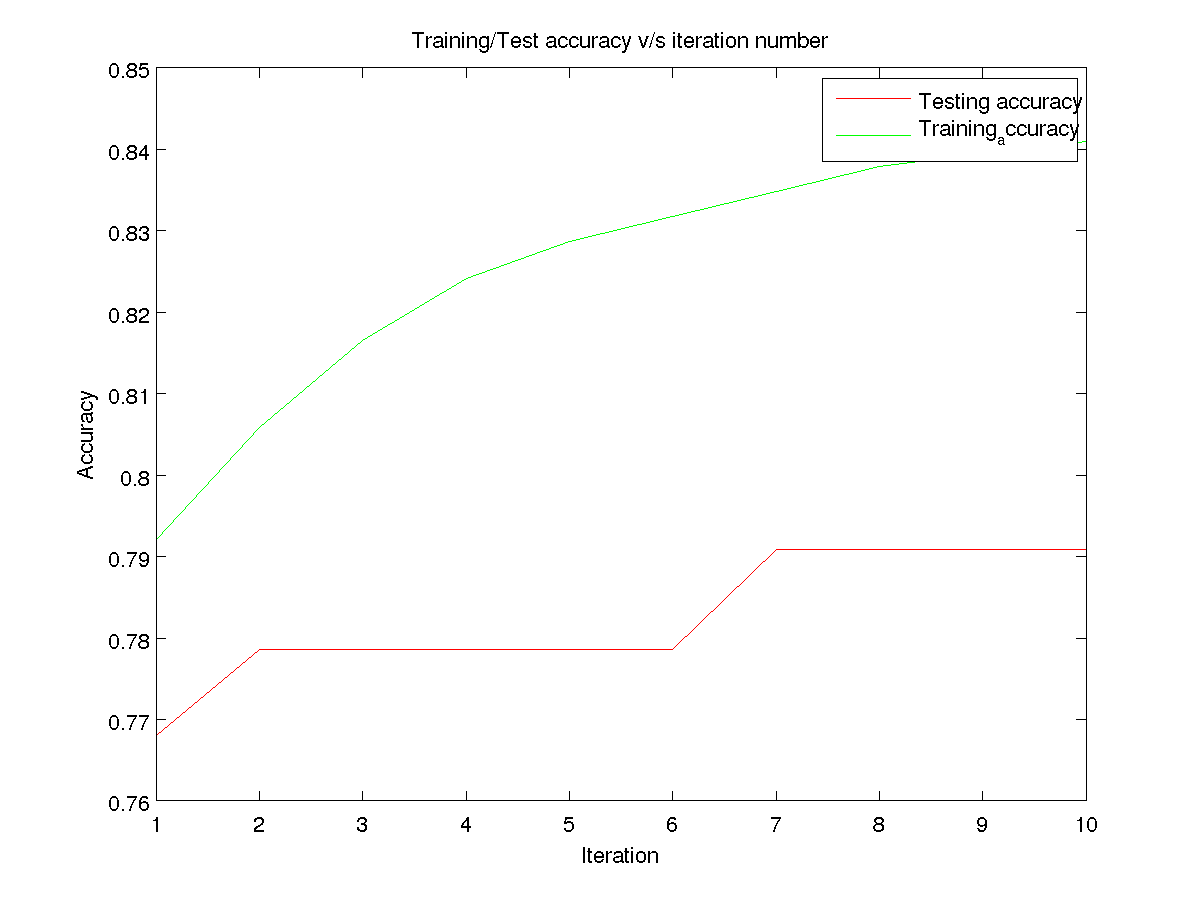
\includegraphics{data/accuracy}
		\caption{4f}
	\end{figure}
	\problemAnswer{
			
			
			The method of forward selection seems to have worked well. The training accuracy increased by increasing the number of features iteratively. This also lead to an increase in test accuracy though only marginally.
			As evident, the training accuracy plot seems to flatten (and hence saturate) near 0.85 for around 10 features. So $10$ features can be assumed to be an optimal choice for number of features.
			
		}
\end{homeworkSection}

\begin{homeworkSection}{\homeworkProblemName: ~(g)}

	
	Alpha: 1.000000e-03     Iterations to Converge:  4862   Accuracy: 7.022901e-01\\
	Alpha: 2.000000e-03     Iterations to Converge:  6114   Accuracy: 7.423664e-01\\
	Alpha: 3.000000e-03     Iterations to Converge:  5807   Accuracy: 7.843511e-01\\
	Alpha: 4.000000e-03     Iterations to Converge:  5731   Accuracy: 8.015267e-01\\
	Alpha: 5.000000e-03     Iterations to Converge:  5393   Accuracy: 8.091603e-01\\
	Alpha: 6.000000e-03     Iterations to Converge:  5192   Accuracy: 8.187023e-01\\
	Alpha: 7.000000e-03     Iterations to Converge:  4914   Accuracy: 8.339695e-01\\
	Alpha: 8.000000e-03     Iterations to Converge:  4730   Accuracy: 8.473282e-01\\
	Alpha: 9.000000e-03     Iterations to Converge:  4624   Accuracy: 8.454198e-01\\
	Alpha: 1.000000e-02     Iterations to Converge:  4513   Accuracy: 8.454198e-01\\
	Alpha: 1.100000e-02     Iterations to Converge:  4371   Accuracy: 8.492366e-01\\
	Alpha: 1.200000e-02     Iterations to Converge:  4218   Accuracy: 8.549618e-01\\
	Alpha: 1.300000e-02     Iterations to Converge:  4102   Accuracy: 8.625954e-01\\
	Alpha: 1.400000e-02     Iterations to Converge:  4036   Accuracy: 8.645038e-01\\
	Alpha: 1.500000e-02     Iterations to Converge:  4024   Accuracy: 8.664122e-01\\
	Alpha: 1.600000e-02     Iterations to Converge:  4078   Accuracy: 8.721374e-01\\
	Alpha: 1.700000e-02     Iterations to Converge:  4198   Accuracy: 8.740458e-01\\
	Alpha: 1.800000e-02     Iterations to Converge:  4366   Accuracy: 8.759542e-01\\
	Alpha: 1.900000e-02     Iterations to Converge:  4564   Accuracy: 8.797710e-01\\
	Alpha: 2.000000e-02     Iterations to Converge:  4760   Accuracy: 8.835878e-01\\
	Alpha: 2.100000e-02     Iterations to Converge:  4897   Accuracy: 8.835878e-01\\
	Alpha: 2.200000e-02     Iterations to Converge:  4953   Accuracy: 8.874046e-01\\
	Alpha: 2.300000e-02     Iterations to Converge:  4948   Accuracy: 8.874046e-01\\
	Alpha: 2.400000e-02     Iterations to Converge:  4913   Accuracy: 8.912214e-01\\
	Alpha: 2.500000e-02     Iterations to Converge:  4864   Accuracy: 8.912214e-01\\
	Alpha: 2.600000e-02     Iterations to Converge:  4811   Accuracy: 8.931298e-01\\
	Alpha: 2.700000e-02     Iterations to Converge:  4759   Accuracy: 8.912214e-01\\
	Alpha: 2.800000e-02     Iterations to Converge:  4710   Accuracy: 8.931298e-01\\
	Alpha: 5.000000e-02     Iterations to Converge:  4292   Accuracy: 9.217557e-01\\
	Alpha: 5.100000e-02     Iterations to Converge:  4270   Accuracy: 9.236641e-01\\
	Alpha: 5.200000e-02     Iterations to Converge:  4248   Accuracy: 9.236641e-01\\
	Alpha: 5.300000e-02     Iterations to Converge:  4226   Accuracy: 9.236641e-01\\
	Alpha: 5.400000e-02     Iterations to Converge:  4204   Accuracy: 9.217557e-01\\
	Alpha: 5.500000e-02     Iterations to Converge:  4183   Accuracy: 9.217557e-01\\
	Alpha: 5.600000e-02     Iterations to Converge:  4162   Accuracy: 9.217557e-01\\
	Alpha: 5.700000e-02     Iterations to Converge:  4142   Accuracy: 9.217557e-01\\
	Alpha: 1.300000e-01     Iterations to Converge:  3801   Accuracy: 9.408397e-01\\
	Alpha: 1.310000e-01     Iterations to Converge:  3805   Accuracy: 9.408397e-01\\
	Alpha: 1.320000e-01     Iterations to Converge:  3808   Accuracy: 9.408397e-01\\
	Alpha: 1.330000e-01     Iterations to Converge:  3811   Accuracy: 9.408397e-01\\
	Alpha: 1.340000e-01     Iterations to Converge:  3814   Accuracy: 9.408397e-01\\
	Alpha: 1.350000e-01     Iterations to Converge:  3818   Accuracy: 9.408397e-01\\
	Alpha: 1.360000e-01     Iterations to Converge:  3821   Accuracy: 9.408397e-01\\
	Alpha: 1.370000e-01     Iterations to Converge:  3825   Accuracy: 9.408397e-01\\
	Alpha: 1.380000e-01     Iterations to Converge:  3828  \textbf{  Accuracy: 9.408397e-01}\\
	
	Thus, it takes approximately 4000 iterations to converge with the choice of the slope parameter around 0.1 and gives an accuracy of 0.94. (Also very low values of the slope parameter seems to hit a local minima) It does seem to be converging in a stable way.
	
	\textbf{	glmfit accuracy: 0.984733}
	
\end{homeworkSection}


\begin{homeworkSection}{\homeworkProblemName: ~(h)}
	\problemAnswer{
		N
	}
\end{homeworkSection}


\end{homeworkProblem}

\end{document}
